\documentclass{article}
\usepackage{geometry}
\geometry{margin=1.5cm, vmargin={0pt,1cm}}
\setlength{\topmargin}{-1cm}
\setlength{\headheight}{12.5pt}
\setlength{\paperheight}{29.7cm}
\setlength{\textheight}{25.3cm}

\usepackage[UTF8]{ctex}
\usepackage{fancyhdr}
\usepackage{layout}
\usepackage{luacode}
\usepackage{tikz}
\usetikzlibrary{arrows.meta,positioning}

% % % % % % % % % % % % % % % % % % % % % % % % % % % % % % % %
% Common Macros for LaTeX
% % % % % % % % % % % % % % % % % % % % % % % % % % % % % % % %

% Useful packages
\usepackage{amsfonts}
\usepackage{amsmath}
\usepackage{amssymb}
\usepackage{amsthm}
\usepackage{enumerate}
\usepackage{graphicx}
\usepackage{multicol}
\usepackage[ruled,linesnumbered]{algorithm2e}

% Math operators and common symbols
\newcommand{\dif}{\mathrm{d}}
\newcommand{\innerProd}[1]{\left\langle #1 \right\rangle}
\newcommand{\difFrac}[2]{\frac{\dif #1}{\dif #2}}
\newcommand{\pdfFrac}[2]{\frac{\partial #1}{\partial #2}}
\newcommand{\T}{\mathrm{T}}
\newcommand{\norm}[1]{\left\| #1 \right\|}
\newcommand{\abs}[1]{\left| #1 \right|}

% Vector and Matrix shortcuts
\newcommand{\vecTwo}[2]{
  \begin{bmatrix}
    #1 \\
    #2
\end{bmatrix}}
\newcommand{\vecThree}[3]{
  \begin{bmatrix}
    #1 \\
    #2 \\
    #3
\end{bmatrix}}
\newcommand{\vecTwoH}[2]{
  \begin{bmatrix}
    #1 & #2
  \end{bmatrix}
}
\newcommand{\vecThreeH}[3]{
  \begin{bmatrix}
    #1 & #2 & #3
  \end{bmatrix}
}

% Common fields
\newcommand{\R}{\mathbb{R}}
\newcommand{\C}{\mathbb{C}}
\newcommand{\Z}{\mathbb{Z}}
\newcommand{\N}{\mathbb{N}}

% Solutions and proofs
\newenvironment{solution}{
\begin{proof}[解]}{
\end{proof}}

% Utility to get environment variables (requires lualatex)
\newcommand{\getEnv}[2]{\directlua{tex.print(os.getenv("#1") or "#2")}}


\newcommand{\name}{\getEnv{NAME}{NAME}}
\newcommand{\uid}{\getEnv{UID}{UID}}
\newcommand{\course}{离散数学}
\newcommand{\hwNum}{图论习题}
\newcommand{\dist}{\operatorname{dist}}
\newcommand{\indeg}{\operatorname{indeg}}
\newcommand{\outdeg}{\operatorname{outdeg}}

\tikzset{
  opnode/.style={circle,draw,minimum size=7mm,inner sep=0pt},
  leafnode/.style={circle,draw,minimum size=5mm,inner sep=0pt},
  every picture/.style={line cap=round,line join=round}
}

\begin{document}

\pagestyle{fancy}
\fancyhead{}
\lhead{\name (\uid)}
\rhead{\today}

\section{题目 5.12}

已知 $n$ 阶无向图 $G$ 中有 $m$ 条边，各顶点的度数均为 $3$。
又已知 $2n-3=m$，在同构的意义下，$G$ 是唯一的吗？
若 $G$ 为简单图，是否唯一？

\begin{solution}
  \[
    \sum_{v\in V(G)}\deg v=3n=2m.
  \]
  结合 $m=2n-3$，
  \[
    3n=2(2n-3)=4n-6,
    \qquad n=6,\quad m=9.
  \]

  不唯一。下面两个简单图都满足条件：$K_{3,3}$ 与三棱柱图。
  它们都有 $6$ 个顶点、$9$ 条边，且每个顶点度数均为 $3$。
  但 $K_{3,3}$ 是二部图，不含三角形；三棱柱图含有三角形。
  因而二者不同构。

  \begin{center}
  \begin{tikzpicture}[scale=0.95, every node/.style={circle,draw,inner sep=1.5pt}]
    \node (u1) at (0,1.2) {};
    \node (u2) at (0,0) {};
    \node (u3) at (0,-1.2) {};
    \node (v1) at (2,1.2) {};
    \node (v2) at (2,0) {};
    \node (v3) at (2,-1.2) {};
    \draw (u1)--(v1) (u1)--(v2) (u1)--(v3)
          (u2)--(v1) (u2)--(v2) (u2)--(v3)
          (u3)--(v1) (u3)--(v2) (u3)--(v3);
    \node[draw=none,rectangle] at (1,-1.75) {$K_{3,3}$};

    \begin{scope}[xshift=5cm]
      \node (a1) at (90:1) {};
      \node (a2) at (210:1) {};
      \node (a3) at (330:1) {};
      \node (b1) at (90:1.75) {};
      \node (b2) at (210:1.75) {};
      \node (b3) at (330:1.75) {};
      \draw (a1)--(a2)--(a3)--(a1)
            (b1)--(b2)--(b3)--(b1)
            (a1)--(b1) (a2)--(b2) (a3)--(b3);
      \node[draw=none,rectangle] at (0,-2.25) {三棱柱图};
    \end{scope}
  \end{tikzpicture}
  \end{center}

  所以一般无向图不唯一；即使要求 $G$ 为简单图，也不唯一。
\end{solution}

\section{题目 5.19}

求图 5-26 中从 $b$ 到其余各顶点的最短路径和距离。

\begin{center}
\begin{tikzpicture}[>=Latex,scale=1.05,
  v/.style={circle,draw,inner sep=1.5pt,minimum size=6mm}]
  \node[v] (b) at (0,1) {$b$};
  \node[v] (a) at (1.35,2) {$a$};
  \node[v] (c) at (1.35,0) {$c$};
  \node[v] (e) at (2.8,1) {$e$};
  \node[v] (d) at (4.45,2) {$d$};
  \node[v] (f) at (4.45,0) {$f$};
  \node[v] (g) at (5.95,1) {$g$};
  \draw[->] (b)--node[above left] {$7$} (a);
  \draw[->] (b)--node[below left] {$1$} (c);
  \draw[->] (c)--node[left] {$3$} (a);
  \draw[->] (a)--node[above] {$8$} (d);
  \draw[->,bend left=20] (d) to node[above] {$2$} (a);
  \draw[->] (a)--node[above right] {$2$} (e);
  \draw[->] (c)--node[below right] {$4$} (e);
  \draw[->] (e)--node[above left] {$1$} (d);
  \draw[->] (e)--node[above] {$2$} (g);
  \draw[->] (c)--node[below] {$3$} (f);
  \draw[->] (f)--node[below left] {$4$} (e);
  \draw[->] (d)--node[above right] {$2$} (g);
  \draw[->] (f)--node[below right] {$7$} (g);
  \draw[->,bend right=45] (f) to node[right] {$10$} (d);
\end{tikzpicture}
\end{center}

\begin{solution}
  对源点 $b$ 用 Dijkstra 算法。各顶点被确定的顺序及距离为
  \[
    c:1,\qquad a:4,\qquad f:4,\qquad e:5,\qquad d:6,\qquad g:7.
  \]
  最短路径整理如下：
  \[
  \begin{array}{c|c|c}
    \text{终点} & \text{最短路径} & \text{距离}\\ \hline
    c & b\to c & 1\\
    a & b\to c\to a & 4\\
    f & b\to c\to f & 4\\
    e & b\to c\to e & 5\\
    d & b\to c\to e\to d & 6\\
    g & b\to c\to e\to g & 7
  \end{array}
  \]
\end{solution}

\section{题目 6.7}

图 6-28 所示各图中哪些是欧拉图？

\begin{center}
  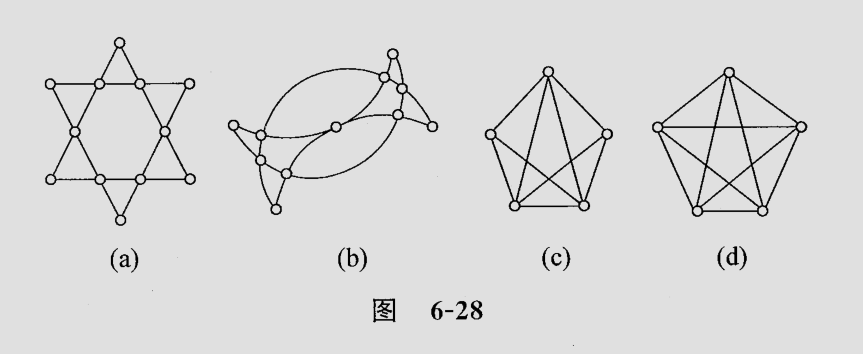
\includegraphics[width=0.82\textwidth]{6-28.png}
\end{center}

\begin{solution}
  连通无向图为欧拉图，当且仅当所有顶点度数都是偶数。

  逐图数度：
  \begin{itemize}
    \item (a) 连通，且各顶点度数均为偶数，是欧拉图；
    \item (b) 连通，重边逐条计数，环贡献 $2$，各顶点度数仍为偶数，是欧拉图；
    \item (c) 左、右两个侧顶点度数为 $3$，不是欧拉图；
    \item (d) 为 $K_5$，每个顶点度数为 $4$，是欧拉图。
  \end{itemize}
  故欧拉图为 (a)、(b)、(d)。
\end{solution}

\section{题目 6.18}

一座楼房底层的建筑平面图如图 6-29 所示。
能否从南门进入，北门离开，走遍所有的房间且每个房门恰好经过一次？

\begin{center}
  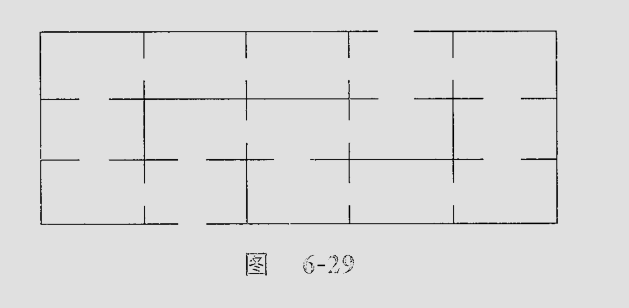
\includegraphics[width=0.62\textwidth]{6-29.png}
\end{center}

\begin{solution}
  以房间为顶点、门为边，把平面图化为房间邻接图。
  从南门进、北门出并且每个门恰好走一次，就是要求这个邻接图存在一条指定端点的欧拉通路。

  欧拉通路要求奇度顶点恰好为两个，并且这两个奇度顶点就是起点和终点。
  按图中门洞逐房间数度，除南门、北门所在房间外仍有奇度房间。
  奇度顶点超过两个，故不存在所要求的走法。
\end{solution}

\section{题目 6.19}

指出图 6-30 所示平面图各面的次数，并验证各面次数之和等于边数的 $2$ 倍。

\begin{center}
\begin{tikzpicture}[scale=0.95, every node/.style={circle,draw,inner sep=1.5pt}]
  \node (l) at (0,0) {};
  \node (t) at (0.8,0.8) {};
  \node (r) at (1.6,0) {};
  \node (b) at (0.8,-0.8) {};
  \node (m) at (2.8,0) {};
  \node (s) at (3.7,-0.55) {};
  \node (u) at (4.7,0.45) {};
  \node (w) at (5.7,0.05) {};
  \draw (l)--node[above left,draw=none,rectangle] {$e_1$} (t)
        (t)--node[above right,draw=none,rectangle] {$e_2$} (r)
        (r)--node[below right,draw=none,rectangle] {$e_3$} (b)
        (b)--node[below left,draw=none,rectangle] {$e_4$} (l);
  \draw (r)--node[above,draw=none,rectangle] {$e_5$} (m);
  \draw (m)--node[below,draw=none,rectangle] {$e_6$} (s);
  \draw (s) edge[loop below,min distance=12mm] node[draw=none,rectangle] {$e_7$} (s);
  \draw (s)--node[below,draw=none,rectangle] {$e_8$} (w)
        (w)--node[right,draw=none,rectangle] {$e_9$} (u)
        (u)--node[left,draw=none,rectangle] {$e_{10}$} (s);
  \node[draw=none,rectangle] at (0.8,0) {$R_1$};
  \node[draw=none,rectangle] at (3.7,-1.05) {$R_2$};
  \node[draw=none,rectangle] at (4.75,0.05) {$R_3$};
  \node[draw=none,rectangle] at (3.25,0.7) {$R_0$};
\end{tikzpicture}
\end{center}

\begin{solution}
  图中共有 $10$ 条边，记外部面为 $R_0$，其余三个内部面为 $R_1,R_2,R_3$。
  各内部面的次数为
  \[
    \deg R_1=4,\qquad \deg R_2=1,\qquad \deg R_3=3.
  \]
  这里 $R_2$ 由环 $e_7$ 围成，次数为 $1$。

  外部面 $R_0$ 的边界中，左侧菱形贡献 $4$，桥边 $e_5,e_6$ 各贡献 $2$，
  环 $e_7$ 的外侧贡献 $1$，右侧三角形贡献 $3$。所以
  \[
    \deg R_0=4+2+2+1+3=12.
  \]
  于是各面次数之和为
  \[
    \deg R_0+\deg R_1+\deg R_2+\deg R_3
    =12+4+1+3=20=2\cdot 10=2|E|.
  \]
\end{solution}

\section{题目 7.8}

求图 7-23 所示两个带权图的最小生成树，并计算它们的权。

\begin{center}
\begin{tikzpicture}[scale=0.95, every node/.style={circle,draw,inner sep=1.5pt,minimum size=5mm}]
  \node (ul) at (0,1.2) {};
  \node (ur) at (2.6,1.2) {};
  \node (br) at (2.6,-1.2) {};
  \node (bl) at (0,-1.2) {};
  \node (o) at (1.3,0) {};
  \draw (ul)--node[above,draw=none,rectangle] {$3$} (ur)
        (ur)--node[right,draw=none,rectangle] {$6$} (br)
        (br)--node[below,draw=none,rectangle] {$1$} (bl)
        (bl)--node[left,draw=none,rectangle] {$5$} (ul);
  \draw (ul)--node[above left,draw=none,rectangle] {$1$} (o)
        (ur)--node[above right,draw=none,rectangle] {$2$} (o)
        (bl)--node[below left,draw=none,rectangle] {$3$} (o)
        (br)--node[below right,draw=none,rectangle] {$4$} (o);
  \node[draw=none,rectangle] at (1.3,-1.8) {(a)};

  \begin{scope}[xshift=6cm]
    \node (t) at (1.5,1.35) {};
    \node (l) at (0,0) {};
    \node (r) at (3,0) {};
    \node (x) at (0.65,-1.35) {};
    \node (y) at (2.35,-1.35) {};
    \draw (t)--node[above left,draw=none,rectangle] {$1$} (l)
          (t)--node[above right,draw=none,rectangle] {$2$} (r)
          (l)--node[above,draw=none,rectangle] {$3$} (r)
          (x)--node[below,draw=none,rectangle] {$8$} (y)
          (l)--node[left,draw=none,rectangle] {$7$} (x)
          (r)--node[right,draw=none,rectangle] {$7$} (y)
          (l)--node[below right,draw=none,rectangle] {$6$} (y)
          (x)--node[below left,draw=none,rectangle] {$5$} (r);
    \draw (x) to[bend right=55] node[left,draw=none,rectangle] {$4$} (t);
    \draw (t) to[bend right=55] node[right,draw=none,rectangle] {$4$} (y);
    \node[draw=none,rectangle] at (1.5,-1.95) {(b)};
  \end{scope}
\end{tikzpicture}
\end{center}

\begin{solution}
  \textbf{图 (a).}
  设四个角点依次为左上 $u_1$、右上 $u_2$、右下 $u_3$、左下 $u_4$，
  中心点为 $v$。
  Kruskal 算法依次取
  \[
    u_4u_3(1),\quad u_1v(1),\quad vu_2(2),\quad vu_4(3).
  \]
  这四条边连通全部 $5$ 个顶点且无圈，权为
  \[
    1+1+2+3=7.
  \]

  \textbf{图 (b).}
  设上顶点为 $t$，左、右中点为 $l,r$，左、右下点为 $x,y$。
  先取
  \[
    tl(1),\quad tr(2).
  \]
  边 $lr(3)$ 构成圈，舍去。再取两条权为 $4$ 的外侧边 $tx(4),ty(4)$。
  因而可取最小生成树
  \[
    \{tl,tr,tx,ty\},
  \]
  总权
  \[
    1+2+4+4=11.
  \]
\end{solution}

\section{题目 7.14}

图 7-26 给出的二叉树表达一个算式。
\begin{enumerate}[(1)]
  \item 给出这个算式的表达式；
  \item 给出算式的波兰符号法表达式；
  \item 给出算式的逆波兰符号法表达式；
  \item 设 $a=4,b=3,c=1,d=3,e=3,f=1,g=2,h=3,i=2,j=1$，
    分别用波兰符号法表达式和逆波兰符号法表达式计算这个算式。
\end{enumerate}

\begin{center}
\begin{tikzpicture}[level distance=12mm,
  level 1/.style={sibling distance=54mm},
  level 2/.style={sibling distance=31mm},
  level 3/.style={sibling distance=21mm},
  level 4/.style={sibling distance=15mm},
  level 5/.style={sibling distance=10mm}]
  \node[opnode] {$+$}
    child {node[opnode] {$/$}
      child {node[opnode] {$-$}
        child {node[opnode] {$*$}
          child {node[opnode] {$+$}
            child {node[leafnode] {$a$}}
            child {node[opnode] {$*$}
              child {node[leafnode] {$b$}}
              child {node[leafnode] {$c$}}}}
          child {node[leafnode] {$d$}}}
        child {node[leafnode] {$e$}}}
      child {node[opnode] {$+$}
        child {node[leafnode] {$f$}}
        child {node[leafnode] {$g$}}}}
    child {node[opnode] {$*$}
      child {node[opnode] {$*$}
        child {node[leafnode] {$h$}}
        child {node[leafnode] {$i$}}}
      child {node[leafnode] {$j$}}};
\end{tikzpicture}
\end{center}

\begin{solution}
  \begin{enumerate}[(1)]
    \item 按中序遍历读出
      \[
        \frac{((a+bc)d-e)}{f+g}+hij.
      \]

    \item 前序遍历得到波兰表达式
      \[
        +\; /\; -\; *\; +\; a\; *\; b\; c\; d\; e\; +\; f\; g\; *\; *\; h\; i\; j.
      \]

    \item 后序遍历得到逆波兰表达式
      \[
        a\; b\; c\; *\; +\; d\; *\; e\; -\; f\; g\; +\; /\; h\; i\; *\; j\; *\; +.
      \]

    \item 代入
      \[
        a=4,\ b=3,\ c=1,\ d=3,\ e=3,\ f=1,\ g=2,\ h=3,\ i=2,\ j=1,
      \]
      得
      \[
        \frac{((4+3\cdot 1)\cdot 3-3)}{1+2}+3\cdot 2\cdot 1
        =\frac{18}{3}+6=12.
      \]
      用波兰式或逆波兰式按栈计算，结果同为 $12$。
  \end{enumerate}
\end{solution}

\section{题目 7.15}

用一棵二叉树表示下述命题公式，并写出它的前缀符号法表达式和后缀符号法表达式：
\[
  ((p\vee q)\wedge \neg r)\to ((\neg p\wedge q)\to(q\vee r)).
\]

\begin{solution}
  对应的二叉树为
  \[
  \begin{tikzpicture}[baseline=(root.base),level distance=11mm,
    level 1/.style={sibling distance=58mm},
    level 2/.style={sibling distance=34mm},
    level 3/.style={sibling distance=20mm}]
    \node[opnode] (root) {$\to$}
      child {node[opnode] {$\wedge$}
        child {node[opnode] {$\vee$}
          child {node[leafnode] {$p$}}
          child {node[leafnode] {$q$}}}
        child {node[opnode] {$\neg$}
          child {node[leafnode] {$r$}}}}
      child {node[opnode] {$\to$}
        child {node[opnode] {$\wedge$}
          child {node[opnode] {$\neg$}
            child {node[leafnode] {$p$}}}
          child {node[leafnode] {$q$}}}
        child {node[opnode] {$\vee$}
          child {node[leafnode] {$q$}}
          child {node[leafnode] {$r$}}}};
  \end{tikzpicture}
  \]

  前缀式为
  \[
    \to\ \wedge\ \vee\ p\ q\ \neg\ r\ \to\ \wedge\ \neg\ p\ q\ \vee\ q\ r.
  \]

  后缀式为
  \[
    p\ q\ \vee\ r\ \neg\ \wedge\ p\ \neg\ q\ \wedge\ q\ r\ \vee\ \to\ \to.
  \]
\end{solution}

\end{document}
